\documentclass[a4paper,12pt]{scrartcl}

\usepackage[utf8]{inputenc}
\usepackage[T1]{fontenc}
\usepackage{lmodern}

\usepackage{graphicx}
\usepackage{subfig}
\usepackage{pdfpages}
\usepackage{float}

% one-and-a-half line spacing as specified in the assessment description
\usepackage{setspace}
\onehalfspacing

% The package to configure the enumerate environment
\usepackage{enumitem}

\usepackage{url}

\usepackage[left=2cm,right=2cm,top=2cm,bottom=3cm]{geometry}

\renewcommand{\baselinestretch}{1.50}\normalsize
  
\begin{document}


\title{Webshop for Baby Clothes}
\subtitle{Human Computer Interaction Course 2011}
\date{\today}
\author{Alban Edouard, Gianin Basler, Irem Tanriseven, Joana Welti}
\maketitle

\tableofcontents

\newpage

% The introduction, containing the description of the designed system.
\section{Introduction}
This document describes the design of our baby clothes selling system. Our system is implemented as a web shop and allows customers to order baby clothes online. 

Each of the sections represent the milestones as presented in the lecture.

This document was written with Latex and is hosted on GitHub~\footnote{\url{https://github.com/joanawelti/Human-Computer-Interaction-Project-AGIJ}}

% Description of users and personas (max. 2 pages)
\section{Description of users and personas}
\subsection{Users and characteristics}

In our web application, there are mainly three types of users which are parents' grandparents and relatives and friends. We choose them as users because parents want to buy baby clothes to their babies' grandparents need to buy baby clothes to their grandchilds also relatives and friend prefer buying bay clothes as gifts to new parents.

\subsubsection{Parents}

Parents are between age of 16 and 50. They use shop more often than other users so they are frequent users. They have less domain experience particularly if they are new parents. They more need to buy baby clothes therefore they may prefer to buy cheaper clothes

\subsubsection{Grandparents}

Grandparents are between 50 and 99 They know about children in other words they have more domain experience. 
They do not use internet often so they need more help about the system. They tend to spend more money on baby clothes.

\subsubsection{Relatives and friends}

Relatives and friends are between 16 and 50. They do not know about children if they are not parents. They look for a gift so they tend to spend more money on baby clothes. They are not frequent users for this web shop, but they most likely have used web shops before.


\subsection{User Groups}
We identified three different user groups for our web shop, based on our own experiences with online shopping.
 
\subsubsection{Frequent users}
Frequent users use the web store on a regular basis. This user group mainly consists of parents, which need new clothes for their babies from time to time, as children grow out of their clothing quite fast in the first couple of years. Also, parents might need clothes for more than one child.

Frequent users know their way around the web site and are familiar with the checkout process. In order to speed up ordering, it is possible to create an account, which allows frequent users to save their shipping address and to review previous orders.

\subsubsection{First time/infrequent users}
First time or infrequent users don't know the web site yet, but have used web shops before. This group includes relatives, maybe also some grandparents, who are looking for a present for the parents and their baby. They might not want to register, so they should be provided the possibility to order without having to create an account.
 
\subsubsection{Users not accustomed to using web shops}
This user group mainly consists of grandparents, looking for clothes for their grandchildren. This user group doesn't use the internet often and needs extra assistance in ordering. Help/explanation texts and and easy and intuitive navigation are essential for this user group. 

\subsection{Personas}
\textbf{Jeff and Judy Seavers}
Aged 63 and 60, have just become grand parents for the first time, as their daughter Julie just gave birth to a little girl.
They have two children themselves. Jeff is a car mechanic while Judy learned dress making but stopped working just before they had their first child.
Both are capable of using a computer but don't use the Internet often, except for writing e-mails to their children.
They have never used an online shop before and thus need all the assistance they can get to navigate through the shop. For their picture, please refer to figure \ref{fig:seavers}.	

\textbf{Main idea}:
Grandparents, never used a web shop before, but with good domain knowledge. Not likely to become registered users, as they seldom buy baby clothes.

\textbf{Sarah Gordon}
Single mother, aged 28. Has had her first child two years ago and awaits her second. She is recently divorced and lives alone at the time being.
She is a teacher at the local high school and knows her way around computers. 
She enjoys spending as much time with her child. She only works 60\% and has to live on a tight budget. At least once a month she goes out with two of her best friends to hit the local clubs. Online shops are nothing new to her as she often shops online so she does not have to leave her child unattended or take him along to the store.
For her picture, please refer to figure \ref{fig:gordon}.	


\textbf{Main idea}:
Persona belonging to the parent category. Has good domain and also computer knowledge and is already a registered user.

\textbf{Bruce Walker}:
Bruce is a social worker living in London. He is 42 years old and is married, but without children.
His youngest sister Tracie has had a baby almost three years ago. He himself likes travelling too much to settle down and have children at the moment.
He seldom uses online shops, as he does not really like the idea of buying goods online. But he has used different webshops a few times. For his picture, please refer to figure \ref{fig:walker}.	


\textbf{Main idea}:
Middle-aged persona with some indirect domain knowledge. Some computer knowledge is present, but he is a new user to the site.

\textbf{Greg Campbell}:
He is studying Philosophy at the University of Aberdeen in his second year. Greg is 20 years old.
His best friend Lisa, aged 22, just had her first child and he is really excited to buy some clothes for her baby.
Greg met Lisa at the University, as she is studying Philosophy, too. He had a crush on her since freshers week but was too shy to ask her out.
He often uses computers for his studies and regularly uses a couple of online shops, mainly to buy some new gadget.

\textbf{Main idea}:
A frequent web shop user, but new to this particular web shop. Has no domain knowledge but will probably register, due to his liking of online shops.

% Task analysis and scenarios (max. 2 pages)
\section{Task analysis and scenarios}

\subsection{Hierarchical tasks model}

For create our tasks, we have analyze different websites for baby clothes, like \textit{oshkoshbgosh.com} or \textit{mybabyclothesboutique.com}, but also websites for adults clothes (\textit{fashion.warehouse.co.uk}, etc).

\subsubsection{Buy baby clothes}
\begin{enumerate}[label*=\arabic*.,start=0,itemsep=-4pt]
  \item In order to buy baby clothes in the Web shop :
  \item Find an item 
    \begin{enumerate}[label*=\arabic*.,itemsep=-4pt]
      \item Search for a specific item (by name or reference)
      \item Brows through all items
				\begin{enumerate}[label*=\arabic*.,itemsep=-4pt]
				  \item Sort by category, price, name, size or availability
        \end{enumerate}
    \end{enumerate}
  \item Select an item and get more details for it
  \item Add item to the shopping cart
    \begin{enumerate}[label*=\arabic*.,itemsep=-4pt]
      \item Select size, color and quantity
    \end{enumerate}
  \item See items in shopping cart
    \begin{enumerate}[label*=\arabic*.,itemsep=-4pt]
      \item Delete items
      \item Change quantity, size or color for all items
    \end{enumerate}
  \item Go to check out
    \begin{enumerate}[label*=\arabic*.,itemsep=-4pt]
      \item Confirm shopping items or delete items
      \item Log in with an user name and a password (or create a new account or continue without account)
      \item Select address and name
	\begin{enumerate}[label*=\arabic*.,itemsep=-4pt]
	  \item Choose a personal data set among all personal data 
	  \item Provide personal data (name, street, city, country, phone number, email address)
        \end{enumerate}
      \item Select payment method
      \item Confirm order      
    \end{enumerate}
  \item Log out
\end{enumerate}
Plan 1 : repeat 2-3-4-5-6 in this order for all different purchases that you need\\
Plan 2 : do (2.a) or (2.b) ; (2.b.i) is not mandatory\\
Plan 6 : do (6.b) if not already logged ; do (6.b), (6.c.i) and (6.f) only if user account exist ; in (6.b) three possibilities : log in, create a new account (go to ``create a customer account'' task) or continue without account ; do (6.c.ii) if new personal data or for user not logged\\

\subsubsection{Create a customer account}
\begin{enumerate}[label*=\arabic*.,itemsep=-4pt]
  \item In order to create a customer account :
  \item Provide an user name and a password
  \item Provide personal data (name, street, city, country, phone number, email address)
  \item Save account
\end{enumerate}
Plan 1 : do 2-3-4 in this order\\
Plan 2 : repeat 2 until user name entered is not yet in use

\subsubsection{Manage an account}
\begin{enumerate}[label*=\arabic*.,itemsep=-4pt]
  \item In order to manage a customer account :
  \item Log in with an user name and a password
  \item Look at history of orders
  \item Change personal data
    \begin{enumerate}[label*=\arabic*.,itemsep=-4pt]
      \item Edit data
      \item Save data
    \end{enumerate}
  \item Go to special offers page
\end{enumerate}
Plan 1 : do 2 in first and after do 3-4-5 independently\\
Plan 5 : go to ``buy baby clothes'' task (2.b) but with special offers

\subsection{Scenarios}
\textbf{Jeff and Judy Seavers} would like to surprise their daughter with a complete set of baby clothes.
Because Julie just had a girl, they would like to buy primarily pink or red clothes. Cost isn't that important, since they will be a present for their daughter.
They would like to get the ordered clothes before their daughter leaves the hospital in about four days, so they need to be able to learn how to navigate through the online shop as quickly as possible.

\textbf{Sarah Gordon} still has most of the baby clothes from her first
child. She only needs a new romper suit.
Due to the fact that she does not have much money, the romper suit should be as cheap as possible.
But because she wants her child to look cute, she would like to find a suit with a hood and attached ears.

\textbf{Bruce Walker} is on the lookout for some nice baby clothes to give to his niece for her third birthday.
He doesn't really know what he wants but he always thinks that babies in yellow clothes look particularly cute, so he would like to buy yellow clothes.
Because his sister's baby will have her first birthday in about 2 weeks, he needs to have the clothes until then.

\textbf{Greg Campbell} would really like to buy a suit for Lisa's son. But after a couple of talks with Lisa, he realised that a shirt and some pants would be better suited.
He likes prints on his shirts, so he would like to find a shirt with the words "Rock Star" printed on it.
Finding a nice shirt is more important to him than the price, but he wishes not to spend more than \pounds20 at the moment, including delivery.

% User involvement methos (Questionnaires/Inquiries) (max. 3 pages)
\section{User Involvement Methods}
In order to find out more about our future users, we decided to design a questionnaire and to do a contextual inquiry. 

\subsection{Questionnaire}
Questionnaires are simple to administer and an easy way to get to know about the general attitude people have about buying clothes online, baby clothes in particular. Since we are building a web shop, our target group has access to a computer and an email account, so we designed our questionnaire in a way that it can be sent out by email. Our questions aim at finding out more about our users, their online shopping behavior as well as their previous experiences with web shops. 

We conducted our study in two phases. First, we designed a draft to do a pilot study to get some feedback from users. Then, we improved our questionnaire according to this feedback and did the actual study with the final version of the questionnaire. To explain what the questionnaire is all about, we wrote an accompanying email, which can be found in the appendix section ~\ref{sec:letter}

\subsubsection{First Draft}
The questionnaire starts with an explanatory section on how to answer the multiple-choice questions, followed by some personal information inquiries, questions about web shops, online clothes stores in general and baby clothes stores in particular. It ends with a disclaimer on the usage of the questionnaire.

The \textit{personal information} questions aim at finding out more about the person filling out the questionnaire. With these questions, we want to find with what kind of person (parent, age, experience etc.) we are dealing with. The \textit{web shops in general} section tries to find out more about the person's online shopping behavior. Especially, we would like to know if people mind to create an account when ordering items online, if wishlists are a feature that is actually used and what other features are valued most by users.
We also ask some more specific questions concerning clothes web shops to find out what the problems are when buying clothes online so that we can enhance our shop with features to make it easier to buy clothes online. 
Last, we have a few questions about \textit{baby clothes shops} in particular. We would like to include the feature that people can buy and sell used clothes online and we would like to know if users consider this useful. Also, we aren't sure how much help people need when deciding on the right size for baby clothes, so we have another question concerning selecting the correct size.

The first draft was designed by three members of our group.

\subsubsection{Pilot study}
In order to test the questionnaire, we handed it out to the forth member of our group to see what he thinks about it, being a computing science student and having attended the Human Computer Interaction Course as well. He also gave the questionnaire to .. (TODO) other people.

After the pilot tests, the questionnaire was updated with some improvements our team mate suggested. Also, some mistakes were corrected. In the introduction part, we added a simple question for the example in addition to the response. For the questions 3 and 12.a, instead of repeating the previous question, we just wrote "if yes", which is clearer. The fourth question was entirely rewritten because some people didn't understand the "computing expertise" term. In questions 6 and 10, "store" was replaced "shop" to keep the terminology consistent. The last update was the inversion (question 11) of the scale of values, from 1 = "not useful" to 5 = "very useful", because this seems to be more natural to people.

\subsubsection{Results}
We sent out .. questionnaires and got ... responses.


\subsection{Inquiry}
With our Contextual Inquiry, we wanted to find out what kind of problems people have when buying baby cloths online. Since our system is a greenfield engineering project, we didn't have a system at hand to let users work with. Therefor, we decided to use OshKosh B'Gosh~\footnote{http://www.oshkoshbgosh.com/}, a website we consider to be quite nice.
%We designed some questions to ask our inquiry volunteers first, some tasks to perform on the OshKosh B'Gosh website, questions to ask afterwards and some key features we as observers should pay attention to.
The inquiry consists of first questions, three tasks to perform by the inquired person, key features to look out for as an observer, and questions to ask afterwards.

The \textit{first questions} are designed to find out some background information about our inquired person in terms of their previous experiences with web shops. 
%Since we could't actually let them do the entire checkout process, we also asked a question about preferred payment method and creating accounts for shops. 

Our \textit{task descriptions} ask the inquired person to perform three different tasks. The first one has its focus on finding an item as cheap as possible, where the second one asks for a very specific item. The third task is based on the second one and was included to find out if our users are familiar with the shopping cart concept. 

While our inquired person does our tasks, we want to see how they find the products we ask them to find in order to learn more about how people navigate on a web shop. We also want to look for if the ``filter by'' and the search functionality is used to find out how we can include them in the most useful way in our project. 

The \textit{questions afterwards} focus on the experience the inquired person had.

The inquiry plan can be found in section~\ref{sec:contextual_inquiry}.

\subsubsection{Results}




% Information Architecture (max. 3 pages + 1 page)
\section{Information Architecture}

\subsection{Organisation Structure}
Our web application has a Hybrid Organization Structure. In this type of organization structure there is a relation between the hierarchical model and the underlying database. We are planning to use this type of organization since in our system, there is a hierarchy between the web pages and there should be a database system in it.

\begin{figure}[ht!]
  \centering  
  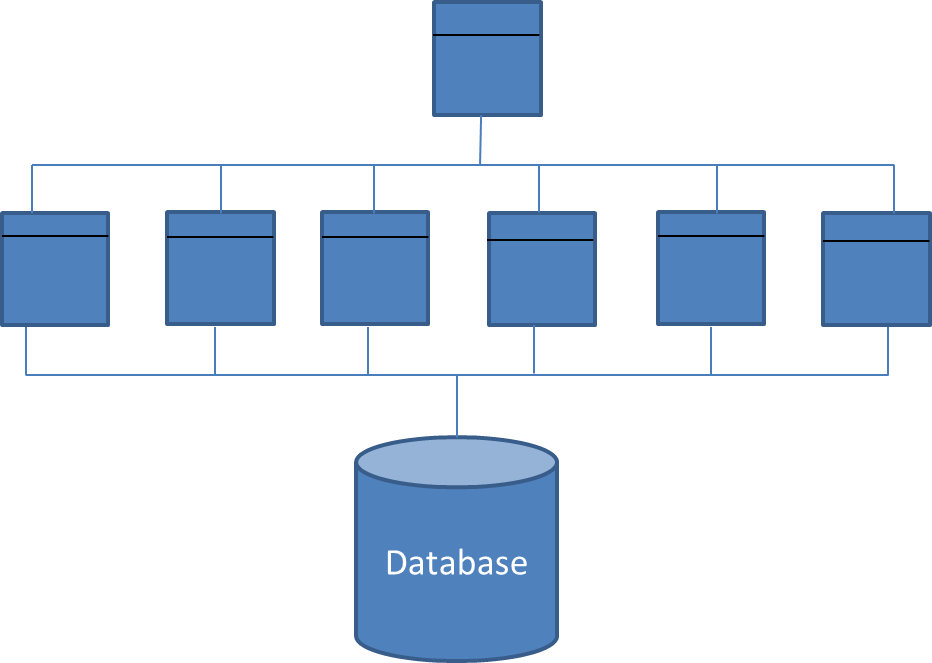
\includegraphics[width=0.5\textwidth]{Images/hybrid_org.png}                
  \caption{Hybrid Organisation Structure}
  \label{fig:hybrid_org}
\end{figure}


\subsection{Organisation Scheme}
Our system has an Inexact Organisation Scheme. The users are able to find the items by means of topic. It is beneficial for particularly the first time users who may not know what they are searching or users who wish to browse through the available products. This scheme is also useful to provide a search.

\subsection{Labeling System}\label{sec:labeling_system}
We aim to develop a user-friendly web application, therefore it is important to have specific and clear labels. To determine the labels which are used in our web application, we looked at some websites selling baby clothes such as \textit{oshkoshbgosh.com} and \textit{babymallonline.com}.

\begin{itemize}
\item In our application, there are a reasonable number of categories. 
\item Each category has some members. 
\item In order to determine the labels, we analyzed the existing webshops.
\end{itemize}

We have different 
% TODO: what do you mean with groups?
groups 
for baby boys and baby girls, because these two groups have different types of clothes. The users generally try to find an item by means of the type of the clothes, so we have labels for different types of baby clothes. 
% TODO: base on inquiry results, not on questionnaire
We reached this result after analyzing the questionnaire results. Also there are two other labels which are clearance and second hand, users are able to look through these pages in order to find some cheaper items.
We use some other subgroups under the main groups so that user are able to find the items they want. 
% TODO: not the only labels
These labels are tops, bottoms, footwear. Under these subgroups, users can look through the type of clothes.

\subsubsection{Labels}
\begin{itemize}
\setlength{\itemsep}{-3pt}
\setlength{\parskip}{0pt}
\setlength{\parsep}{0pt}
 \item Boy 
 \item Girl 
 \item Clearance 
 \item Second Hand
\end{itemize}

\minisec{Boy}
\begin{itemize}
\setlength{\itemsep}{-3pt}
\setlength{\parskip}{0pt}
\setlength{\parsep}{0pt}

	 \item Tops
	 	\begin{itemize}
\setlength{\itemsep}{-3pt}
\setlength{\parskip}{0pt}
\setlength{\parsep}{0pt}
		 \item Shirts and Tees
      	 \item Jackets
      	 \item Sweaters and Hoodies
		\end{itemize}
     \item Bottoms
	 	\begin{itemize}
\setlength{\itemsep}{-3pt}
\setlength{\parskip}{0pt}
\setlength{\parsep}{0pt}
		 \item Trousers
		 \item Jeans
		 \item Shorts
		\end{itemize}
	 \item Footwear
	 	\begin{itemize}
\setlength{\itemsep}{-3pt}
\setlength{\parskip}{0pt}
\setlength{\parsep}{0pt}
		 \item Boots
		 \item Sneakers
		 \item Sandals
		 \item Socks
		\end{itemize}
	 \item Bodysuits	
     \item Pajamas
	\end{itemize}

\minisec{Girl} 
\begin{itemize}
\setlength{\itemsep}{-3pt}
\setlength{\parskip}{0pt}
\setlength{\parsep}{0pt}

	 \item Tops (same as for Boy)
     \item Bottoms
	 	\begin{itemize}
\setlength{\itemsep}{-3pt}
\setlength{\parskip}{0pt}
\setlength{\parsep}{0pt}
		 \item Trousers
		 \item Jeans
		 \item Shorts
		 \item Skirts
		\end{itemize}
	 \item Dresses 
	 \item Footwear (same as for Boy)
	 \item Bodysuits	
     \item Pajamas
	\end{itemize}
\minisec{Clearance and Second Hand} 
\begin{itemize}
\setlength{\itemsep}{-3pt}
\setlength{\parskip}{0pt}
\setlength{\parsep}{0pt}

	 \item Tops
	 	\begin{itemize}
\setlength{\itemsep}{-3pt}
\setlength{\parskip}{0pt}
\setlength{\parsep}{0pt}
		 \item Shirts and Tees
      	 \item Jackets
      	 \item Sweaters and Hoodies
		\end{itemize}
     \item Bottoms
	 	\begin{itemize}
\setlength{\itemsep}{-3pt}
\setlength{\parskip}{0pt}
\setlength{\parsep}{0pt}
		 \item Trousers
		 \item Jeans
		 \item Shorts
		 \item Skirts
		\end{itemize}
	 \item Dresses
	 \item Footwear
	 	\begin{itemize}
\setlength{\itemsep}{-3pt}
\setlength{\parskip}{0pt}
\setlength{\parsep}{0pt}
		 \item Boots
		 \item Sneakers
		 \item Sandals
		 \item Socks
		\end{itemize}
	 \item Bodysuits	
     \item Pajamas
	\end{itemize}



% Navigation (max. 1 pages)
\section{Navigation}
%Relevant? ->
%As our website will be used by cell phones or computers, it is important to develop a design which supports user navigation, printing, etc. For this reason, we use a single-screen design and navigation tools.

\subsection{General design}

Nowadays, there are a lot of devices which are able to access websites and each of them has a different screen size. It is better to use a single-screen design than a predefined size of screens (for example 800x600). It assures that the navigation is usable on various devices. 

It is also important to establish a compromise between separate pages and scrolling on a long page. Users don't like to scroll pages, but if there are too many pages, user can get lost in the number of different pages.

\subsection{Global systems}

We place our logo at the top on the left side. The logo is included on every subpage to ensure that the user always knows on which website he is.
At the top of every page and directly to the right of the website logo, the global navigation menu can be found. As defined in \ref{sec:labeling_system}, the menu (figure \ref{fig:globalMenu} in the appendix) is composed of the followings groups: Boy, Girl, Clearance and Second Hand.

\subsection{Local systems}\label{sec:local_systems}
The local menu appears, as a cascading menu, when the user moves the mouse on one of the global menu items. It is also on the left of every page (except the home page) below the logo and the global menu. As soon as the user selects one of the entries, he has access to the subgroups of this category, as defined in \ref{sec:labeling_system}. For most subgroups, users can also select a subsubgroup in the cascading menu. Figure \ref{fig:localMenu} shows examples for the Boy's local menu on the left, it can be found in the appendix.

\subsection{Contextual and Supplemental systems}
Hypertext links or associative links will be provided within the textual description to a selected item. There are "also bought" and "you may also like" lists, with which users can see what other people bought with the selected product, or what the underlying database recommends. Users can also use supplemental navigation tools like the "Search bar" and "Breadcrumbs", which are very useful for finding where they are and offer quick access to specific items.




% Prototype (max. 1 pages)
\section{Prototype}

For represented our prototype, we have designed a series of screen sketches contained in Powerpoint slides. Because we would like an easy to change (by designers or by users), to create and to simulate the prototype, we have decided to implement it in a low fidelity. The Powerpoint slides are in the appendix (slide 1 to 15).

\subsection{Find and select an item}
The first slide shows the home page of our website. By clicking on one of the buttons representing the global systems menus (on the top), the user can accessed to the corresponding local systems menus (as defined in the section \textit{6.3}) and thus access to the slides showing the items. Here, he has the possibility to sort the items using the "Order by" lists, and clicking and the "Go" button, and/or to select one of them. If there are many pages containing items, he can browse each of them thanks to the "Previous" and "Next" buttons (on the bottom). Use the "Search bar", and click on "Find", is another way for finding a specific item. \\

When the user selects an item, a new page appears with its description (price, picture, size, etc). After have added an item in his cart, "Add to cart" button, he can buy it.

\subsection{Buy an item}
When the user want to buy his items, he has to select the "Cart" button (as defined previously, be logged is not mandatory). Thus, he has an overview of each item and can choose its quantity, colour and size. He can then continue his shopping, "Continue shopping" button, or proceed to payment, "Checkout" button. \\

From now, we suppose that the customer doesn't want to be register and has selected "Checkout". The Checkout page is then shown (slide 10) and he has to select "Guest Checkout". From the step 1 to 3 of his Checkout, he must to fill his shipping and payment informations. The final step is to review and place his order. If everything is correct, the confirmation page is shown (slide 15).


% Analytical Usability Evaluation (max. 3 pages)
\section{Analytical Usability Evaluation}
To make sure that our system would be usable in the end, two of our group members acted as experts to perform a Cognitive Walkthrough, while the third person additionally performed a KLM Analysis. We decided on these techniques, because in our opinion a Cognitive Walkthrough will reveal most of the inefficencies and problems in the design of our website, while a KLM Analysis will show how well the webshop is actually designed.
The results of these evaluations are summed up in the following subsections. The complete results can be found in the appendix.

\subsection{Cognitive Walkthrough Setup}
To make sure that the results of the cognitive walkhtrough that our two experts conducted, will be comparable, we chose the following scenario as a starting point:\\

Susan, 82 years old, would like to buy trousers online. Her niece Pam gave birth to an adorable girl just three months ago. Since Susan is invited to go over to Pam's place for dinner, she would like to bring along a present for her. Pam's mentioned that her girl just grew out of another pair of trousers, so Susan would like to get her a new one. She would like to order a nice one, but it should't be too pricey. Susan knows that Pam likes yellow, which is why the trousers should be yellow if possible.

And these are additional assumptions:\\
Susan got her first computer two years ago, but she doesn't use it very often. She's ordered groceries online before, but she's never ordered anything from our shop. She doesn't like to create accounts and always pays with credit card, where possible.

\subsection{Results of the Cognitive Walkthrough}
Two of the more important problems that both experts found were:
\begin{itemize}
	\item User must have some familiarity with web shops to know what the cart is used for
	\item The "next step button" when choosing the payment method should be removed
\end{itemize}
The first problem could be addressed by providing a help feature that walks the user through the order process. This could be done with a simple textual description, or even with a small video that shows how to use the web shop. This would especially be helpful for first time users.
The "next step button" could easily be removed in a final system, by using JavaScript to advance the order process. However, a "back button" would have to be provided to return to the selection of the payment method, in case the user accidentally chooses the wrong method.

Another problem found, lies in the use of the terminology. Although all the webshops we looked at, group "Trousers" under "Bottoms", this might not be evident to everyone. Especially for someone who has never used a clothes webshop before, this might be confusing. To solve this problem, the complete local navigation menu could be displayed at all times. Thus, all entries would be shown for all categories. However, this might not be optimal, since the menu then offers too many options at once. Better options would probably be, either to include a section about the terminology in a help feature, or to show all submenus as soon as the user's mouse is placed over a menu entry.

Most of the other problems that the two experts found are concerned with the ease of navigation and clarity, such as:
\begin{itemize}
	\item Cart doesn't show the number of items in it
	\item User shouldn't be able to click on "Add to cart" without selecting a color/size/quantity above zero
	\item It is not possible to remove an item from the cart
\end{itemize}
Of course, all of these problems would have to be addressed, if the system would actually be implemented. By using JavaScript, or adding a few buttons and drop-down lists to the design, these problems could easily be handled.

Overall, the design seems to be quite reasonable. Some mistakes were found, but none of them are very serious. However, only a user test with a final, implemented system could show, if the users can really navigate the system, as we intend it.

\subsection{Key-Level Model Analysis Setup}

% User Testing (max. 3 pages)
\section{User Testing}

%TODO introduction

\subsection{What we want to find out in our test}
How fast can users perform certain tasks?
Tasks:
\begin{itemize}\addtolength{\itemsep}{-0.5\baselineskip}
	\item Buy a pair of yellow trousers for a girl of 6 months.
	\item Create an account for themself.
\end{itemize}
We would like to find out if an experienced user is faster than a beginner, in performing these tasks.

Additional questions:
\begin{itemize}\addtolength{\itemsep}{-0.5\baselineskip}
	\item Do the user find the right controls? How many mistakes do they make?
	\item Do the users like the design and layout of the webshop? And why?
\end{itemize}
We are employing the "summative evaluation" technique.


\subsection{The types of users we would like to use for our test}
To make sure that the test will give meaningful results, we would like to have at least 30 users with the following aspects, evenly distributed over our user groups:
\begin{itemize}\addtolength{\itemsep}{-0.5\baselineskip}
	\item Users who see a web shop for the first time
	\item Users who are experienced with buying things online
\end{itemize}
These are the groups of users we are looking for:
\begin{enumerate}\addtolength{\itemsep}{-0.5\baselineskip}
	\item Young user (around 20) with much computer experiences
	\item Middle age (around 40) with much and also with few experiences
	\item Older (around 60) with few experiences
\end{enumerate}
To find users within the first group, we would go to different universities, ask lecturers if it's possible to conduct a small pre-test with their students. To do this, we would create groups of people and for each group give them a short task, watch them and select the people that are most suitable for the test.
To find test subjects, for the second and third group we would like to use teachers and staff of different universities. And perform the same pre-test, as for the first group, to make sure that we have suitable candidates.
Finally, we would use the "matched pairs design" because it will be easy to match pairs within our test user groups. We also expect order effects to be significant, since more experienced users will be able to solve our tasks much more quickly.

Instructions for the test:\\
Just try to do the task and take your time. If you have any questions, please ask a member of the supervisors.

\subsection{Test location}
We will perform our test in a lab. It is easier to perform the test in a lab, than to go to people's homes and because we would like to use observational equipment. Also, if we provide the computer to run the test on, we make sure that everyone will use the same computer. Additionally, we don't want to put our website online, until it is really finished. Thus, it won't be possible to let people do the test at home.

\subsection{Observational methods}
We will both gather quantitative and qualitative data.  The time to complete our set task, the amount of errors the users make and the number of button presses, necessary to order an item in our webshop, or to create an account i the quantitative data we wish to gather. This data can then be compared to our findings from the Key-Level-Mapping Analysis. The qualitative data will then tell us where the problems lie and what problems the users have. In order to determine this, we will take notes to accompany the video that we will take while performing the test. These notes will include detail about possible confusions, hesitations, or mistakes of the users and the exact page and subtasks where they occurred. This can then be compared to the Analytical Usability evaluation, performed by our experts.
We will encourage the users to think aloud and comment what they are doing. This will also give us an insight in the difficulties that the users have.

\subsection{Questionnaire for after the test}
%TODO 
Are you going to use a questionnaire for after the users have finished their tasks?
Yes


What questions will you ask? 
Have you enjoyed the test?
Have you had any problems?
Did you find all relevant information? If no, why?
Will you recommend this website to anyone else? And why?




\section{Appendix}
\subsection{Personas}

\begin{figure}[h!]
  \centering
  \subfloat[Jeff and Judy Seavers]{\label{fig:seavers}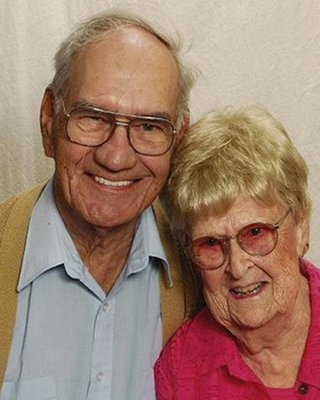
\includegraphics[width=0.3\textwidth]{Images/jeff_and_judy_seavers.jpg}}                
  \subfloat[Sarah Gordon]{\label{fig:gordon}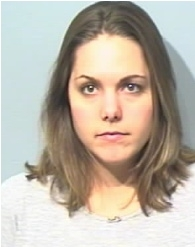
\includegraphics[width=0.3\textwidth]{Images/sarah_gordon.jpg}}
  \subfloat[Bruce Walker]{\label{fig:walker}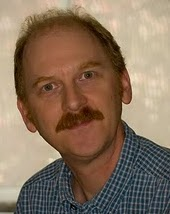
\includegraphics[width=0.3\textwidth]{Images/bruce_walker.jpg}}
  \caption{Personas}
  \label{fig:personas}
\end{figure}

\subsection{User Involvement Methods}
\subsubsection{Accompanying letter}\label{sec:letter}
Dear \dots

For our course ``Human Computer Interaction'', we have to design a system for selling baby clothes. Our group decided to build a web-based system, for which we need your help. In order to find out about which features our system should include, we made a questionnaire with some questions concerning web shops (in general and clothes/baby clothes in particular).
If you can spare fifteen minutes of your time, we'd greatly appreciate if you could help us and fill out the questions.

Thank you very much!\\
Alban Edouard, Gianin Basler, Irem Tanriseven, Joana Welti


\subsubsection{Questionnaires}

Why the Prototype files appear before the questionnaires ???

\begin{figure}[h!]
\centering
\includegraphics[width=1.0\textwidth]{User_Involvement_Methods/Questionnaires/Questionnaire_Web_Shops_v2.pdf}
\end{figure}

\begin{figure*}[h!]
\centering
\includegraphics[width=1.0\textwidth]{User_Involvement_Methods/Questionnaires/Questionnaire_Web_Shops_v2_2.pdf}
\caption{Questionnaire First Draft}
\label{fig:draft}
\end{figure*}


\begin{figure*}[h!]
\centering
\includegraphics[width=1.0\textwidth]{User_Involvement_Methods/Questionnaires/Questionnaire_Web_Shops_v3.pdf}
\end{figure*}

\begin{figure*}[h!]
\centering
\includegraphics[width=1.0\textwidth]{User_Involvement_Methods/Questionnaires/Questionnaire_Web_Shops_v3_2.pdf}
\caption{Questionnaire Final Version}
\label{fig:final}
\end{figure*}

\subsubsection{Prototype}
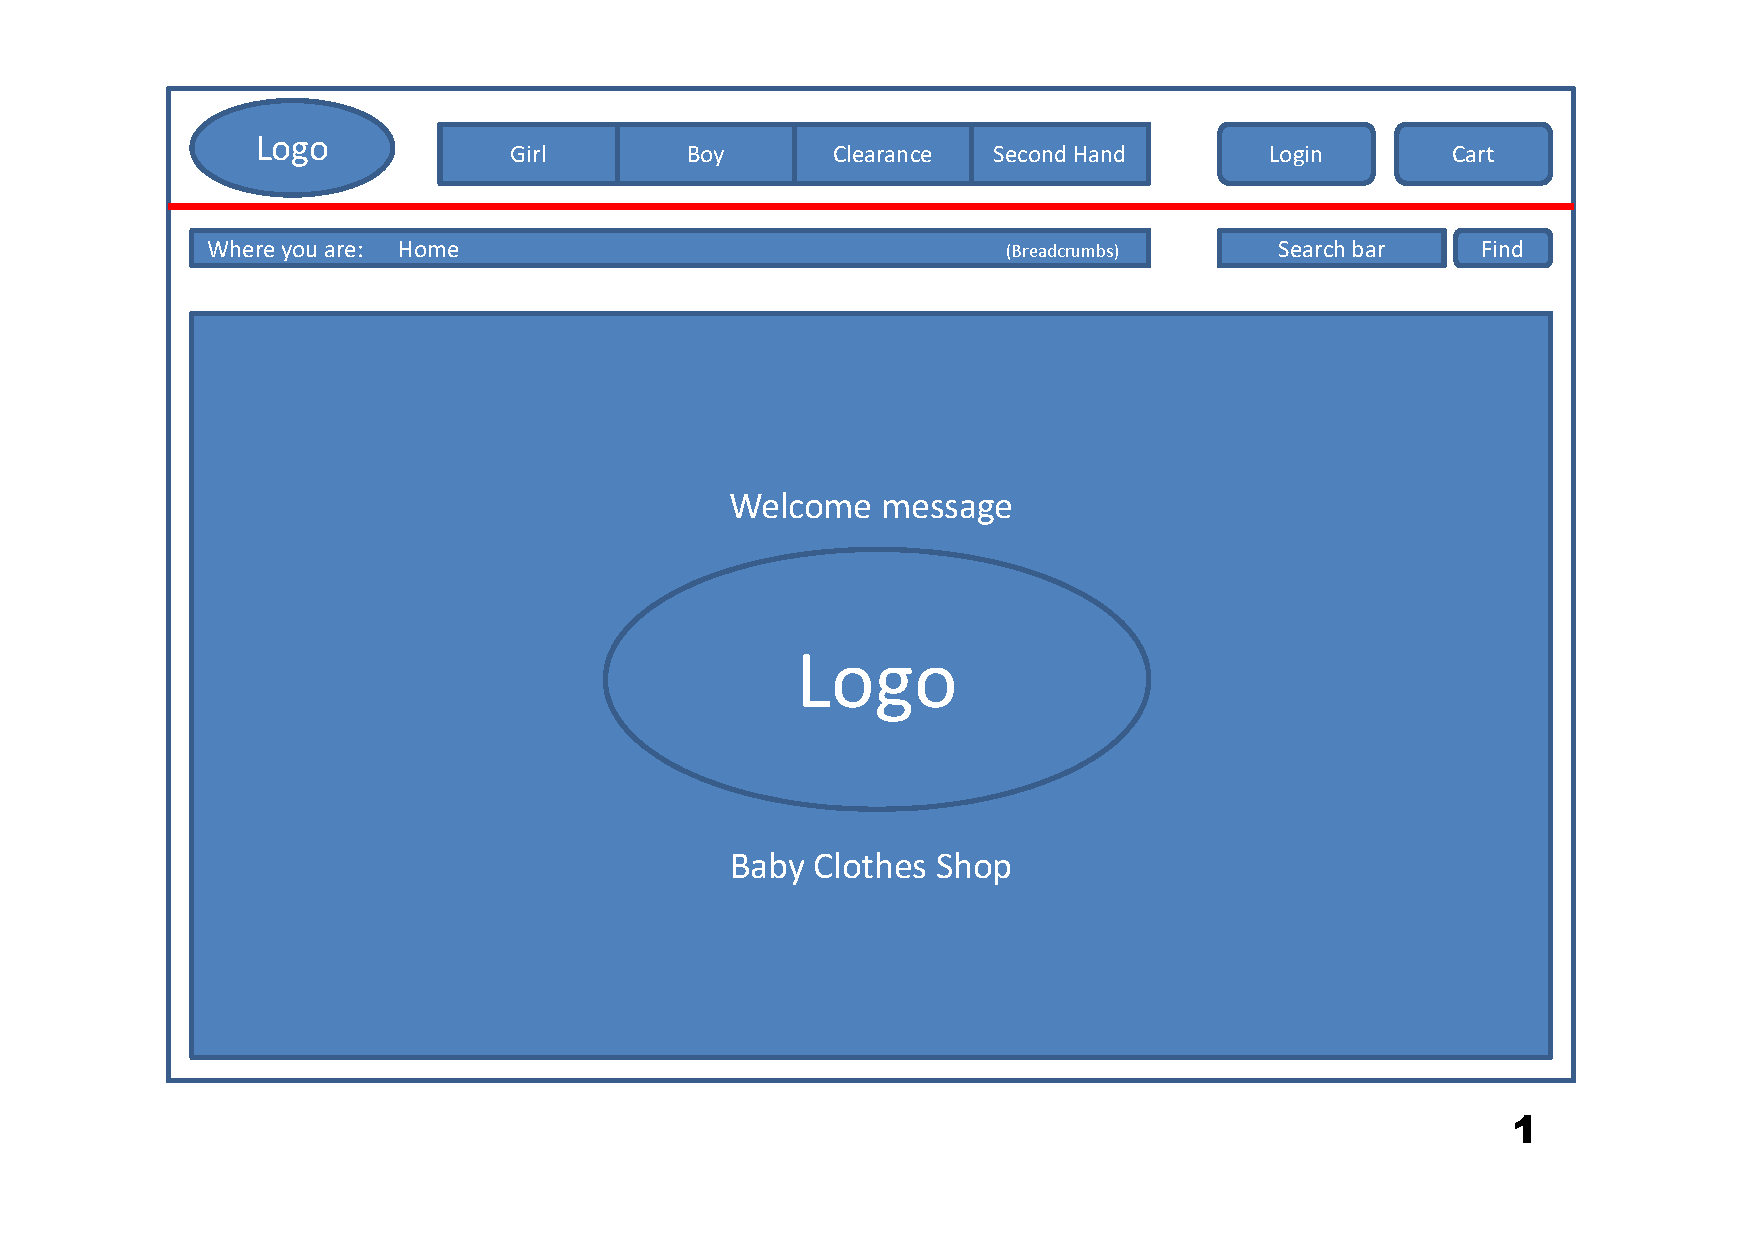
\includepdf[pages=-]{Prototype/HCI_Prototype_2.pdf}




\end{document}